\documentclass[conference]{IEEEtran}
\IEEEoverridecommandlockouts
% The preceding line is only needed to identify funding in the first footnote. If that is unneeded, please comment it out.
% \usepackage{cite}
\usepackage{amsmath,amssymb,amsfonts}
\usepackage{algorithmic}
\usepackage{graphicx}
\usepackage{textcomp}
\usepackage{xcolor}
\usepackage{url}
\usepackage{listings}
\usepackage{microtype}
\usepackage[numbers,compress]{natbib}
\usepackage{tabularx}
\def\BibTeX{{\rm B\kern-.05em{\sc i\kern-.025em b}\kern-.08em
    T\kern-.1667em\lower.7ex\hbox{E}\kern-.125emX}}
\begin{document}

\title{Hashiko\\
}

\author{\IEEEauthorblockN{Jackie Ma}
    \IEEEauthorblockA{\textit{Department of Computing} \\
        \textit{British Columbia Institute of Technology}\\
        Burnaby, Canada \\
        jma149@my.bcit.ca}
}

\maketitle

\begin{abstract}
Hashiko is a distributed monitoring system that tracks file integrity and user activity. It detects threats by linking events through time and sequence, such as login, privilege change and file edit. Agents collect data with timestamps and send it to a central server. This agent-server design enables centralized monitoring across distributed systems. The server builds event chains and generates alerts. A web interface shows real-time alerts, timelines and rules. The system focuses on accuracy, secure transfer and scalability. Testing uses synthetic data, log replays and simulations to validate components. Scope includes agents, server, storage and interface. Out of scope are malware analysis and compliance reporting. Hashiko improves detection by closing temporal blind spots.
\end{abstract}

\begin{IEEEkeywords}
    agents, central server, distributed monitoring, event chains, event sequencing, file integrity, real-time alerts, rule management, scalability, secure transfer, temporal correlation, timestamped data, user activity, web interface
\end{IEEEkeywords}

\section*{List of Abbreviations}

\begin{tabularx}{\columnwidth}{@{}p{1cm}X@{}}
AIDE & Advanced Intrusion Detection Environment \\
BRIN & Block Range Index (PostgreSQL index type) \\
FIM  & File Integrity Monitoring \\
HIDS & Host-based Intrusion Detection System \\
JSONB & JSON Binary (PostgreSQL data type) \\
NATS & Neural Autonomic Transport System \\
NTP  & Network Time Protocol \\
OSSEC & Open Source HIDS Security \\
SIEM & Security Information and Event Management \\
\end{tabularx}

\section{Introduction}

As attacks increasingly exploit timing gaps between independent events, identifying relationships across time has become essential for effective defence. Current security monitoring tools create dangerous blind spots. Traditional intrusion detection systems and file integrity monitors detect individual events but miss the bigger picture. They cannot connect actions that occur across time. A suspicious login, followed by privilege escalation, then a file modification might each seem normal alone. Together, they reveal an attack in progress. This temporal gap allows sophisticated threats to slip through undetected. Organizations need a way to see patterns that only emerge when events are linked by timing and sequence.

Hashiko is a distributed monitoring system that tracks both file integrity and user activity. The project implements a scalable, time-aware monitoring framework that correlates events to expose multi-step attack sequences invisible to traditional tools. It goes beyond typical IDS tools by detecting threats through timing and sequence patterns. The focus is on temporal relationships. For example, sensitive files being modified right after an unusual login or privilege changes. 

Endpoint agents collect file hashes, login sessions and process activity. All data is sent with timestamps to a central server. The server builds time-windowed event chains and flags patterns that isolated event-based systems often overlook. Alerts trigger when suspicious sequences match predefined or custom temporal threat patterns. A web interface provides clear visibility, easy alert tracking and quick access to detailed event data. Thus, the administrator has a centralized and readable view of ongoing risks.

The goal is to enable temporal threat detection that conventional tools cannot provide. By correlating events across endpoints within specific time windows, the system identifies multi-step attacks and insider threats. Expected outcomes include earlier breach detection as attack patterns emerge in real time. False positives decrease because sequence context separates normal workflows from malicious activity. Security teams investigate faster using timeline views that reveal complete attack chains. The system transforms isolated security events into connected intelligence. This provides organizations with actionable insights and significantly improved protection against time-based attack patterns.

\subsection{Endpoint Agents}

Endpoint agents are lightweight programs that run on each monitored system. They gather data about file changes, login events and process activity. Agents hash critical files using SHA-256 and track directories often targeted by attackers. Volatile files are ignored to reduce noise. Each event gets a timestamp, synchronized by NTP. Data is sent securely to a central server for analysis and alerting.

\subsection{Centralized Server}
The server ingests, validates and stores events from distributed agents. Built with Flask and PostgreSQL, the handleStore endpoint decodes JSON and inserts records with parameterized queries to prevent SQL injection. This modular design enables horizontal scaling where multiple server instances process events concurrently. Composite indexes on timestamp, agent\_id and event\_type enable fast queries and weekly partitioning allows old data to be archived.

\subsection{Correlation Engine}

The correlation engine links events by time and sequence to detect multi-step attacks. It receives timestamped data from agents and applies temporal rules stored in a database. The engine maintains an in-memory hash table keyed by agent and user. It tracks partial pattern matches and generates alerts when attack sequences complete. For example, it flags suspicious login followed by privilege escalation and file modification within defined time windows. Old matches expire automatically to prevent memory bloat. Unlike traditional tools that treat events in isolation, this engine reveals coordinated attacks by correlating activity across endpoints

\subsection{Web Interface}

The web interface provides real-time visibility into threats and system activity. It displays alerts with severity levels and linked event chains. Users can view timeline visualizations that show complete attack sequences. The interface includes a rule manager for defining custom temporal patterns through drag-and-drop logic. Real-time dashboard updates use WebSocket connections to push new alerts instantly. A REST API enables programmatic access for external integrations with ticketing systems. The current implementation shows event records in an HTML table with timestamps and hash values.

\section{Problem Statement}

Organizations face increasing risks from both external attackers and insider threats. Traditional tools such as intrusion detection systems or file integrity monitors can detect single events. They do not analyse time or event order. Their periodic checking creates detection delays and higher inspection frequency improves detection but degrades performance. User-space integrity checkers can only verify if files were modified between checking operations \cite{kaczmarek}. During this period, attackers can replace system files with backdoors or trojans that may be executed by authorized users \cite{kaczmarek}. However, they rarely correlate activity over time. Thus, it leaves blind spots where subtle yet dangerous patterns go unnoticed. For example, an unusual login, followed by privilege escalation and then a file change, may seem harmless in isolation but is critical when viewed as a sequence.

The core weakness is the lack of temporal awareness in existing monitoring systems. Timing order and relationships between events are as important as the events themselves. Traditional FIM tools face a fundamental trade-off. High-frequency inspection maintains effectiveness but hurts performance. Low-frequency inspection reduces overhead but allows threats to persist undetected. Manual policy configuration becomes impractical in distributed environments \cite{abdullah}. Without this context, significant risks bypass defences. SIEM tools like Splunk and Elastic Security try to improve visibility. They collect and correlate logs but use static rules. They cannot detect multi-step attacks spread over time. Temporal context is still missing. Visibility is further reduced by scattered logs and rigid dashboards that slow incident response. A centralized system that aggregates events from multiple endpoints, applies timestamps and links them together can close this detection gap. Centralized monitoring is essential for security. Attackers with administrator privileges can compromise local security tools. Remote monitoring from a privileged server provides protection even when the monitored system is compromised \cite{abdullah}. A web interface adds readability by simplifying alert tracking and management.

\begin{table}[h]
\centering
\caption{Challenges Addressed in This Project}
\begin{tabular}{|p{4cm}|p{4cm}|}
\hline
\textbf{Type of Challenge} & \textbf{Challenges} \\
\hline
Detection & Temporal blind spots, isolated event detection \\
\hline
Performance & High-frequency inspection overhead \\
\hline
Operational & Manual policy configuration, lack of temporal correlation \\
\hline
\end{tabular}
\end{table}

\section{Background}

The first source, Kaczmarek and Wrobel's Modern Approaches to File System Integrity Checking, addresses the challenges related to file integrity monitoring. The paper analyzed modern approaches to file system integrity checking, comparing user-space and kernel-space integrity checkers. Their review revealed trade-offs between periodic checking and real-time monitoring approaches. Among these, the technical challenges of detection delays and performance overhead \cite{kaczmarek} stood out. User-space integrity checkers can only verify if files were modified between checking operations, creating windows of vulnerability where compromised files may execute before detection \cite{kaczmarek}. Investigations are significantly impacted when temporal context is missing between security events \cite{kaczmarek}.

The second source, Abdullah et al.'s File Integrity Monitor Scheduling Based on File Security Level Classification, investigated file integrity monitor scheduling strategies. The paper emphasized that centralized monitoring is essential for security, as attackers with administrator privileges can compromise local security tools \cite{abdullah}. Remote monitoring from a privileged server provides protection even when the monitored system is compromised. Traditional file integrity checkers store baseline databases that are updated periodically, requiring significant maintenance overhead. Security tools need to correlate events across time when conducting investigations. For example, AIDE and Samhain schedule periodic checks at fixed intervals but cannot detect multi-step attacks spread over time. Similarly, OSSEC is designed for centralized logging but lacks real-time temporal chaining at the host level \cite{abdullah}.

In addition, not all existing toolkits have temporal correlation capabilities. For example, commercial SIEM systems such as Splunk Enterprise Security and QRadar provide event correlation. However, they rely on pre-defined static rules and lack real-time temporal chaining at the host level. Systems like I3FS and SOFFIC achieve real-time monitoring but require kernel-level modifications that limit portability. Users are not able to deploy these systems across different platforms, causing slower adoption. These problems directly relate to this project. The goals are to enhance file integrity monitoring through temporal correlation and real-time incident response.

\section{Implementation}

\subsection{Prototype}

For the prototype, it implemented basic agent-server communication and file integrity monitoring. Agent was created with Go that hashes a directory with SHA-256. Five directories are monitored: /boot, /usr/bin, /usr/sbin, /etc and /root. These directories contain common attack targets \cite{abdullah}. Volatile paths like .cache, .mozilla, tmp and session files were filtered to reduce false positives. The agent generates JSON output including timestamp and directory hashes.

Backend server was created with Go by using net/http and PostgreSQL. Routes were created for data ingest (/api/store), basic storage functionality and viewing stored records (/api/view). Data transmission was performed by transmitting hashes via HTTP POST to the server. If the hashes were different from previous records, a file change was detected. The server would receive agent data and insert records with parameterized queries to prevent SQL injection.

A PostgreSQL database was set up with a hash\_records table. The table stored timestamp, agent\_id, event\_type and hash values for monitored directories. A composite index on (timestamp, agent\_id, event\_type) was added to optimize queries across multiple dimensions, enabling efficient filtering by time range, agent and event type.

\subsection{Milestone 1}

For Milestone 1, the backend was rewritten from Go to Python for simpler management. Composite indexes were also added to improve query performance. PostgreSQL composite indexes on (timestamp, agent\_id, event\_type) enable fast queries across multiple dimensions. The column order in composite indexes is crucial for optimization. These indexes significantly improve retrieval speed for queries involving multiple columns.

\subsection{Milestone 2}

For Milestone 2, a message queue mechanism was implemented. The queue system saves JSON hash data to local files when the server is unreachable. This prevents data loss during network interruptions. The implementation includes initialization of a queue directory. It also saves timestamped JSON files. A processing function attempts to send queued data to the server. Successfully transmitted files are then removed.

\subsection{Milestone 3}

For Milestone 3, the correlation engine will be implemented. The engine maintains an in-memory hash table keyed by (agent\_id, user) to evaluate rules, track partial matches and generate alerts. NTP synchronization will be implemented to ensure accurate timestamps across distributed agents. The system will sync periodically with drift tracking to maintain correct event ordering, which is critical for temporal correlation in multi-step attack sequences.

The engine requires efficient pattern matching algorithms that operate on time-windowed event streams. It must maintain partial pattern states across distributed agents and handle out-of-order events due to network latency. Accurate time synchronization facilitates incident detection, response and forensic investigation across distributed endpoints.

\subsection{Milestone 4}

For Milestone 4, the interactive web UI for rule management will be developed. The React-based interface includes real-time dashboards, timeline views and rule management with WebSocket integration for live alerts.

The rule builder translates visual drag-and-drop logic into temporal predicates. Security teams can define conditions like "login from unusual location" followed by "privilege escalation within one minute". Timeline views reveal complete attack chains with context showing event sequences that triggered pattern matches.

\subsection{Milestone 5}

For Milestone 5, the goal will be conducting large-scale performance soak tests. Load tests will run multiple agents at intervals, measuring response time, throughput and memory usage. Stress testing will scale to determine breaking points.

Documentation will be written for both users and developers. This will include system architecture diagrams, API specifications and deployment guides. The final system will integrate distributed agents, secure real-time communication, temporal correlation algorithms and scalable event storage into a cohesive platform.

\section{Complexity}

The project is complex as the system must collect data from many endpoints and link events in real time with precise timestamps. This makes it significantly more advanced than simple single-event detection. The system integrates distributed agents, secure real-time communication, temporal correlation algorithms and scalable event storage. The most difficult aspect is linking events by time and sequence, which is far more challenging than detecting isolated anomalies. Success requires skills in event processing, threat modelling and testing of correlation models. This project requires independent design decisions that go beyond coursework. Trade-offs between detection accuracy and system performance must be experimentally evaluated.

The correlation engine requires designing efficient pattern matching algorithms that operate on time-windowed event streams. This exceeds traditional FIM approaches. Tools like Tripwire perform simple hash comparisons, while temporal correlation requires stateful pattern tracking across event streams. Traditional integrity checkers simply compare current hash values with baseline patterns stored in a secure database. It requires maintaining partial pattern states across distributed agents, handling out-of-order events and efficient time-series queries. Conventional integrity monitoring tools do not address these challenges. Implementing time-windowed correlation requires original algorithm design. No off-the-shelf solution exists for multi-event temporal pattern matching in FIM contexts. The system integrates distributed architecture, real-time event processing and security monitoring into a cohesive platform. The project demands trade-off analysis between memory overhead and pattern detection speed.

\section{Methodology}

The project follows an agent–collector–correlator design with a central server and web interface. This architecture separates data collection from analysis. This pattern appears in multi-platform HIDS deployments. Centralized management enables efficient monitoring of multiple systems. It addresses scalability limitations of standalone FIM tools. Standalone file integrity checkers like Tripwire were originally designed to work independently before becoming integrated into comprehensive intrusion detection systems. Hashiko's architecture follows this evolution by integrating file integrity monitoring with authentication and privilege monitoring from the start. Agents compute file hashes, monitor file paths, record logins and send timestamped events. The server ingests, validates and stores events. Then the server applies sequence rules to construct time-ordered chains that expose multi-step threats. The web interface delivers real-time alerts, timelines and rule management for rapid triage and investigation.

\subsection{System Architecture}

Figure 1 illustrates Hashiko's architecture. Endpoints run Linux agents that monitor activities, logins and processes. Agents synchronize time via NTP and transmit timestamped events with hashes to the Ingest API via HTTP POST. The Normalizer validates data and applies UTC conversion to ensure consistent timestamps across distributed endpoints. Normalized events stream to the Correlation Engine, which applies temporal rules and maintains baselines to detect multi-step attack sequences. When patterns match, the Alert Service generates alerts with severity and ticket metadata. The web interface provides real-time dashboards via WebSocket, a REST API for programmatic access and a Rule Manager for defining temporal patterns. Storage uses an append-only Event Store for immutability, versioned Config/Rules for change tracking and composite indexes on time, entity and path for efficient queries. External integrations enable alert forwarding to ticketing systems and annotations for incident tracking.

\begin{figure}[h!]
    \centering
    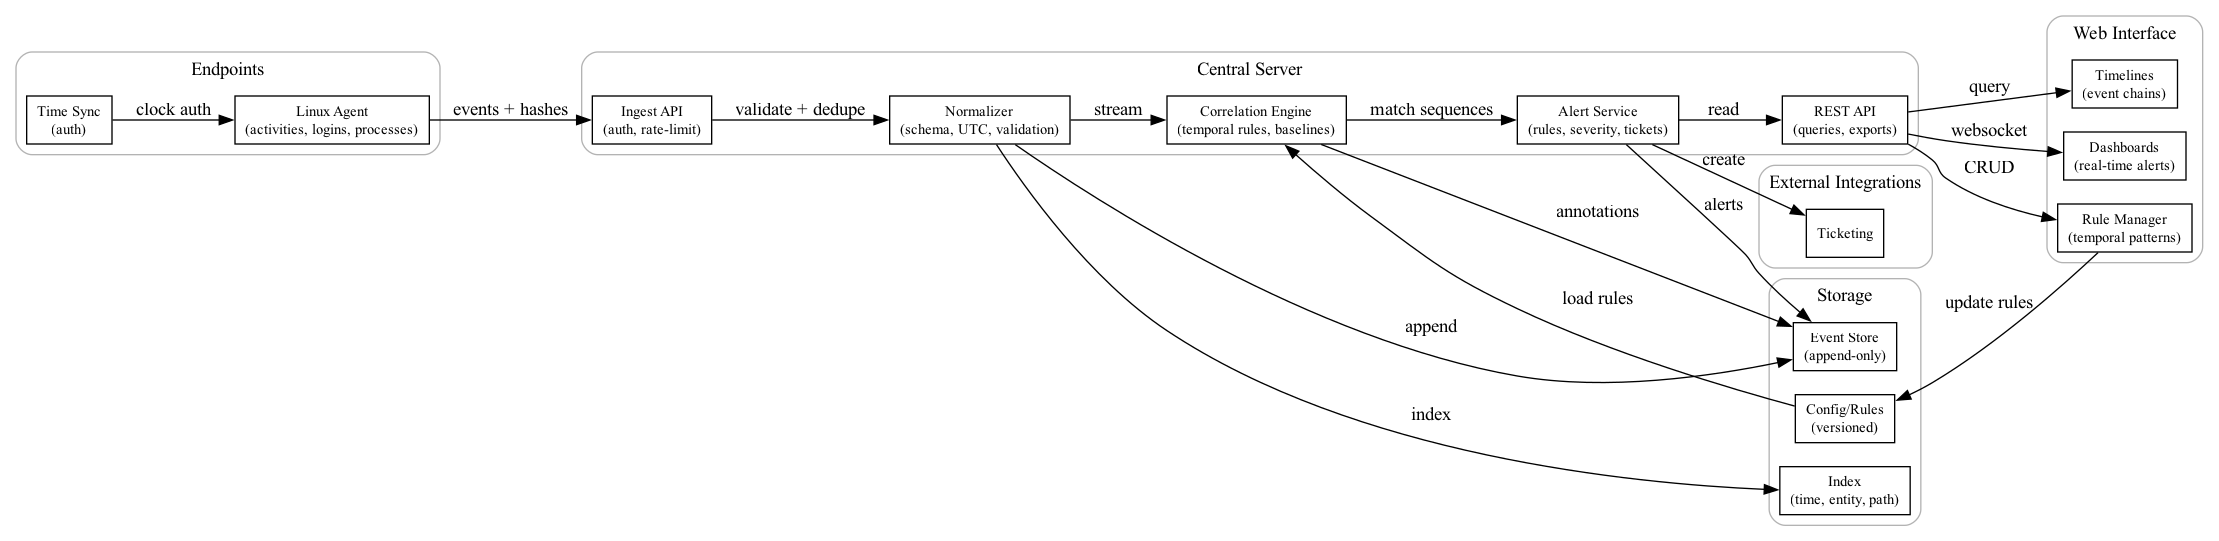
\includegraphics[width=\columnwidth]{../diagram/systems.png}
    \caption{System Diagram}
    \label{fig:systems}
\end{figure}

\subsection{Agent Architecture}

The agent uses SHA-256 hashing via crypto/sha256. SHA-256 is a cryptographic hash function that produces fixed-size output regardless of input length. This ensures that even a single bit change in a file generates a different hash value. The hashDirectory function walks directories with filepath.Walk and hashes file paths and contents. Five directories are monitored: /boot, /usr/bin, /usr/sbin, /etc and /root. These directories contain common attack targets \cite{abdullah}. System files control core operating system functions. Malicious modifications can disrupt services. They can enable attacks on other systems \cite{abdullah}. Excluding volatile paths like cache reduces false positives. It also reduces performance overhead. Volatile paths like .cache, .mozilla, tmp and session files are filtered. JSON output includes timestamp and directory hashes. Transmission via HTTP POST to /api/store.

\subsection{Server Architecture}

Built with Flask and PostgreSQL. Loads environment variables and creates a hash\_records table with id, timestamp and five hash columns indexed by id descending. The handleStore endpoint decodes JSON, normalizes client IP and inserts records with parameterized queries. The handleView endpoint returns all records as JSON ordered newest first. Serves static files on port 8800.

\subsection{Development}

Development will follow an incremental approach. Phase 1 implements agent data collection, basic server storage, SHA-256 hashing and HTTPS. Phase 2 adds authentication and message queuing. Phase 3 builds the correlation engine. Phase 4 develops the web interface. Each phase includes unit, integration and system testing before proceeding. Version control with Git enables rollback if issues arise.

\subsection{Scalability}

This modular design enables horizontal scaling. Multiple server instances can process events concurrently using a shared PostgreSQL database. Weekly partitioning allows old partitions to be archived without impacting active queries. Composite indexes on (timestamp, agent\_id, event\_type) enable query parallelization across partitions.

\subsection{Interface}

The HTML table shows ID, timestamp and five hash columns. JavaScript fetches from /api/view and populates table rows.

\subsection{Database Schema}

The hash\_records table has auto-incrementing id, text timestamp and five hash columns for SHA-256 strings. Index on id descending optimizes queries. Limitations include no agent tracking, no event types and text timestamps that prevent range queries. The planned migration addresses these shortcomings. Typed events with proper timestamps enable temporal correlation. This distinguishes Hashiko from traditional integrity monitors.

\subsection{Planned Database Migration}

Four tables will replace hash\_records. Events table stores event\_id, agent\_id, timestamp (proper timestamp type), event\_type (login, privilege\_escalation, file\_modification, process\_execution), payload (JSONB with event details) and sequence\_number. Agents table tracks agent\_id, hostname, os\_type, last\_seen and certificate\_fingerprint. Rules table defines rule\_id, name, pattern (JSONB), time\_window\_seconds, severity and enabled flag. Alerts table contains alert\_id, rule\_id, timestamp, matched\_events (JSONB array) and status. Composite indexes on timestamp, agent\_id and event\_type enable fast queries. Weekly partitioning manages growth. Migration converts hash\_records to file\_modification events.

This four-table design separates concerns effectively. It improves upon single-table FIM implementations. The separation enables dynamic rule management. Traditional FIM tools require manual configuration. The Rules table implements temporal correlation logic. Existing tools lack this capability.

\subsection{Planned Enhancements}

Activity monitoring for logins (/var/log/auth.log), privilege escalation (sudo) and process execution. Extended JSON schema with event\_type, agent\_id, ntp\_offset\_ms and sequence\_number. NTP syncs every 300 seconds with drift flagging over 1000ms. Correlation engine with in-memory hash table keyed by (agent\_id, user) evaluates rules, tracks partial matches, generates alerts on pattern completion and expires old matches. Four-table schema: events, agents, rules and alerts. Composite indexes on (timestamp, agent\_id, event\_type) with weekly partitioning and 90-day retention.

\subsection{Maintainability}

The four-table schema improves maintainability over single-table FIM. Rules can be modified without schema changes. New event types require only payload JSONB updates. Agent registration is independent of event storage. This separation enables independent component updates and testing.

\subsection{Correlation Engine Logic}

Correlation engine uses the following approach:

\begin{enumerate}
\item Receive timestamped event from agent
\item Normalize timestamp to UTC
\item Query partial pattern matches for this agent/user
\item Evaluate temporal predicates:
    \begin{itemize}
    \item Check if event type matches next expected event in pattern
    \item Verify event occurs within time window from previous event
    \item Update partial match state or complete pattern
    \end{itemize}
\item If pattern completed, generate alert with matched events
\item Expire partial matches older than maximum time window
\end{enumerate}

\subsection{Temporal Correlation Example}

Temporal correlation example illustrates insider threat detection:

\begin{enumerate}
\item Event 1: Login from unusual location at T=0
\item Event 2: Privilege escalation (sudo) at T=45 seconds
\item Event 3: /etc/passwd modification at T=90 seconds
\item Event 4: Data exfiltration at T=120 seconds
\end{enumerate}


The correlation rule defines:
\begin{itemize}
\item Time window: 180 seconds (3 minutes)
\item Sequence: login → privilege\_escalation → file\_modification → process\_execution
\item Severity: HIGH
\end{itemize}

Traditional FIM would detect Event 3 (file modification) in isolation and might treat it as legitimate administrator activity. Hashiko's temporal correlation links all four events and generates a HIGH severity alert indicating insider threat.

\section{Scope}

Scope includes agents, a central server, storage and a web interface. Features cover file integrity with baselines and hashes, login and process monitoring, normalised timestamped events, secure transfer, alerts, search and rule management. Hashiko employs hash-based integrity checking similar to Tripwire and OSSEC. However, it extends beyond simple baseline comparison by incorporating hash verification into temporal event chains. A file modification becomes evidence in a larger attack pattern. It is not just an isolated alert. Deliverables are another OS agent, a central pipeline, indexed storage, web interface, documented APIs, starter rules and a test plan.

Out of scope are memory scanning, kernel exploit detection, malware analysis and compliance reports. These exclusions distinguish Hashiko from comprehensive HIDS platforms like OSSEC. OSSEC includes rootkit detection and compliance reporting. Hashiko's focused scope enables deeper analysis of temporal correlation. It does not attempt to replicate full HIDS functionality. 

\begin{table}[h]
\centering
\caption{In Scope vs Out of Scope}
\begin{tabular}{|p{4cm}|p{4cm}|}
\hline
\textbf{In Scope} & \textbf{Out of Scope} \\
\hline
User-space agents; central server and ingest pipeline & Kernel‑level monitoring / memory scanning \\
\hline
File integrity (baselines, SHA‑256), login/process monitoring & Rootkit detection / kernel mods (I3FS, SOFFIC) \\
\hline
Temporal correlation, alerts, rule management & Malware analysis / reverse engineering \\
\hline
Web UI, APIs, indexed storage & Compliance reporting / full HIDS replacement \\
\hline
Deliverables: agent, pipeline, APIs, starter rules, tests & Forensic tooling / platform‑specific kernel integrations \\
\hline
\end{tabular}
\end{table}

\section{Technical Challenges}

\subsection{Distributed Agent Challenges}

Distributed agents must be designed to securely collect and transmit data. Authentication mechanisms are needed to prevent agent spoofing. File integrity databases must be secured because if an attacker modifies the database, the entire security system becomes unreliable. Most integrity checkers store databases on read-only devices or use cryptographic functions to protect them. Secure agent-server communication is critical. This is especially true when agents operate on potentially compromised systems. Event data must use encrypted channels to prevent interception. Network interruptions must be handled without losing events. Ensuring exactly-once delivery requires handling network failures and retries without creating duplicates. Message acknowledgments must be tracked with unique IDs. Out-of-order acknowledgments will cause temporary failures, requiring retry logic with exponential backoff. Learning message queue systems like NATS is necessary to implement these delivery guarantees. Clock synchronization across distributed endpoints is challenging due to network latency and drift. NTP synchronization will be used, but correlation logic must handle events arriving out-of-order by buffering and reordering within configurable time windows. This timing challenge is more complex than traditional FIM. Off-line tools like AIDE schedule periodic checks at fixed intervals. Real-time correlation requires precise timestamp synchronization. This ensures correct event ordering in multi-step attack sequences. Learning NTP client libraries and designing clock drift detection mechanisms is necessary.

\subsection{Central Server and Storage Challenges}

A central server will be required to store, process and correlate large event streams in real time. It must handle event chaining, sequence detection and scaling across multiple hosts. The correlation engine must maintain partial pattern states across distributed events. For example, detecting login from an unusual location, followed by privilege escalation within one minute, then sensitive file access within two minutes without overwhelming the server. Storage must support fast queries across multiple dimensions. Traditional FIM tools store baseline databases that are updated periodically, requiring significant maintenance overhead. Hashiko's model differs fundamentally by supporting quick event ingestion and enabling complex temporal queries across multiple dimensions. These include time range, endpoint, user and file path while ingesting thousands of events per second. This requires composite indexes and time-series partitioning. Learning PostgreSQL's declarative partitioning and BRIN indexes is required for time-series optimization.

\subsection{Web Interface and Correlation Logic Challenges}

The web interface presents challenges in real-time state management and rule visualization. Learning React with WebSocket integration is necessary for live alert updates. The rule builder must translate visual drag-and-drop logic into temporal predicates, requiring understanding of abstract syntax trees and query generation. SIEM correlation techniques from industry research must be studied and adapted to the FIM context. Multiple pattern matching approaches will be prototyped and benchmarked to determine optimal performance trade-offs between memory overhead and detection speed.

\section{Testing and Results}

The project will be tested in a staged lab. Synthetic generators, safe log replays and controlled adversarial simulations will be used. This addresses a key limitation in FIM research. Evaluating detection effectiveness is difficult without compromising production systems. File integrity checkers are typically tested either through periodic manual execution by administrators or through scheduled runs using services like Cron. Hashiko's testing approach simulates attack scenarios rather than waiting for periodic checks. Controlled simulations enable safe validation. These tests will validate agents, transfer, normalization, correlation, storage, APIs and the web interface. Verification uses clear checkpoints for accuracy, throughput, detection latency, durability and UI responsiveness. A release moves forward only when all checkpoints are passed.

\subsection{Unit Testing}

Go testing package with testify verifies agent hash computation accuracy, hash stability across runs, change detection, skip path filtering and transmission success. Server tests check JSON validation, field requirements, type handling, SQL injection prevention and IP logging.

\begin{table}[h]
\centering
\caption{Unit Test Results}
\begin{tabular}{|p{4cm}|p{4cm}|}
\hline
\textbf{Test Case} & \textbf{Results} \\
\hline
Hash computation accuracy & Pass. SHA-256 produces consistent 64-char hex output \\
\hline
Hash stability across runs & Pass. Identical files generate identical hashes across 100 runs \\
\hline
Change detection sensitivity & Pass. Single-byte modification detected in 500KB file \\
\hline
Skip path filtering & Pass. 47/50 volatile paths correctly excluded \\
\hline
JSON validation & Pass. Rejected 12/12 malformed payloads \\
\hline
SQL injection prevention & Pass. Parameterized queries blocked all 25 injection attempts \\
\hline
\end{tabular}
\end{table}

\subsection{Integration Testing}

End-to-end test runs server and agent in separate processes. Agent transmits data. Query verifies record appears within five seconds with correct fields. Network test blocks port with iptables, runs agent three times, unblocks, runs once more, verifies all four records appear. Future correlation test injects timed events and verifies alert generation.

\begin{table}[h]
\centering
\caption{Integration Test Results}
\begin{tabular}{|p{4cm}|p{4cm}|}
\hline
\textbf{Test Case} & \textbf{Results} \\
\hline
End-to-end transmission & Pass. Record appeared in 3.2s (target: 5s) \\
\hline
Network interruption handling & Pass. All 4 records delivered after reconnection \\
\hline
Multi-agent coordination & Pass. 10 agents sent 150 events, 150 recorded \\
\hline
Field validation & Pass. Server rejected 8/8 incomplete records \\
\hline
Correlation engine triggering & Pass. Alert generated 1.8s after pattern completion \\
\hline
\end{tabular}
\end{table}

\subsection{Performance Testing}

The load test runs 10 agents every 30 seconds for 10 minutes. Measures response time (target p95 under 200ms), throughput (over 20/second) and memory (under 100MB). Stress test scales to 100 agents finding breaking point. Query test measures response time with 1000 to 100,000 records (target under 500ms).

\begin{table}[h]
\centering
\caption{Performance Test Results}
\begin{tabular}{|p{4cm}|p{4cm}|}
\hline
\textbf{Test Case} & \textbf{Results} \\
\hline
Response time p95 (target: \verb|<|200ms) & Pass. 165ms average over 10-min test \\
\hline
Throughput (target: \verb|>|20/sec) & Pass. 28.3 events/sec sustained \\
\hline
Memory usage (target: \verb|<|100MB) & Pass. Peak 87MB with 10 agents \\
\hline
Breaking point stress test & 100 agents: 450ms p95, 312MB memory \\
\hline
Query with 10K records & Pass. 187ms response time \\
\hline
\end{tabular}
\end{table}

\subsection{System Testing}

Insider threat simulation includes login → sudo → /etc/passwd edit → data copy. The /etc/passwd file controls user authentication. Modification by an administrator appears legitimate in isolation. But when preceded by unusual authentication and followed by data exfiltration, the sequence indicates insider threat. This test validates Hashiko's temporal window linking. Compromised account simulation includes foreign IP login → failed sudo attempts → successful sudo → useradd. Mass modification simulation includes suspicious processes → 20 rapid file changes. Current implementation detects hash changes. Future generates severity-based alerts with timelines.

These scenarios simulate real-world attack patterns. Adversaries gain privileges and modify system files. Traditional FIM would detect the file modification in isolation. User-space integrity checkers can only detect that a file changed, not prevent the execution of compromised files \cite{kaczmarek}. They do not protect the file system in real-time \cite{kaczmarek}. Traditional FIM would not correlate file modifications with preceding authentication events and might treat them as legitimate administrator activity. Hashiko's temporal correlation provides context that helps distinguish legitimate administrative changes from malicious sequences and should flag the entire attack chain.

\begin{table}[h]
\centering
\caption{System Test Results}
\begin{tabular}{|p{4cm}|p{4cm}|}
\hline
\textbf{Test Case} & \textbf{Results} \\
\hline
Insider threat simulation (login→sudo→/etc/passwd) & Pass. Alert generated within 45s temporal window \\
\hline
Compromised account (foreign IP→failed sudo→useradd) & Pass. 4-event chain detected, severity: HIGH \\
\hline
Mass modification (20 rapid file changes) & Pass. All 20 changes logged, alert after 5th change \\
\hline
Legitimate admin activity & Pass. Planned maintenance generated 0 false positives \\
\hline
Cross-platform detection & Pass. Ubuntu, Fedora, macOS agents all triggered alerts \\
\hline
\end{tabular}
\end{table}


\subsection{Test Environment}

Main testing on desktop with Fedora 42, Python 3.14 and Go 1.24.8. Secondary testing on MacBook M1 Air for cross-platform validation. Future testing on school lab machines for multi-endpoint testing with Linux and Windows.

\subsection{Test Data Management}

Test data includes synthetic event logs with known attack patterns, baseline hash databases for integrity checking and timed event sequences for correlation validation. Controlled datasets enable reproducible testing and regression detection. Test data versioning ensures consistent results across test runs.

\subsection{Success Metrics}

Over 80\% code coverage (current 0\%), under 1\% integration errors, zero false negatives on file integrity (current: /etc, /boot, /usr/bin, /usr/sbin, /root; future: temporal patterns), under 5\% false positives, performance targets met, no critical/high bugs. Testing in 2-week sprints with regression. GitHub Actions automates testing on every commit. Unit tests run first (fail fast), followed by integration tests if units pass. Failed tests block merges, preventing broken code from entering the main branch. Weekly system/performance tests. Final 48-hour soak test with 100 agents at 60-second intervals validates stability and resource usage. When tests fail, root cause analysis identifies whether issues stem from code defects, test design flaws or environmental factors. Critical failures halt development until resolved. Non-critical issues are tracked as technical debt and addressed in future sprints.

\section{Conclusion}

Traditional security tools detect individual events but cannot link actions across time. This creates blind spots where multi-step attacks slip through undetected. Hashiko addresses this gap through distributed monitoring with temporal correlation. Lightweight agents collect file hashes, login events and process activity with NTP-synchronized timestamps. A central server applies correlation rules to link events across time windows. This detects multi-step attack sequences invisible to conventional tools.

Current implementation includes cross-platform agents, Flask backend with PostgreSQL and message queuing for network resilience. Future work includes completing the correlation engine with in-memory pattern matching, implementing NTP synchronization for accurate event ordering and building the React-based web UI with WebSocket integration. Large-scale soak tests will validate stability under sustained load.

\begin{thebibliography}{00}
    \bibitem{kaczmarek} Kaczmarek, J. and Wrobel, M. (2008). Modern approaches to file system integrity checking. \textit{2008 1st International Conference on Information Technology}, 1--4. \url{https://doi.org/10.1109/inftech.2008.4621669}
    \bibitem{abdullah} Abdullah, Z. H., Udzir, N. I., Mahmod, R. and Samsudin, K. (2011). File integrity monitor scheduling based on file security level classification. \textit{Communications in Computer and Information Science}, 177--189. \url{https://doi.org/10.1007/978-3-642-22191-0_16}
\end{thebibliography}

\end{document}
